Metal/oxide interfaces are among the most important heterogeneous structures because various thin films are present in optical coatings, semiconductor devices, and catalysts. Therefore it is important to understand the thin film stability and morphology evolution during deposition processes. From this study, we will understand: (1) What are the major factors that affect metal thin film morphology during the deposition? (2) How do we improve the wettability of metallic thin films on the oxide substrates?

To answer these two questions, \ac{GCMC} simulations are conducted on various substrates based on Ag-substrate bonding strength obtained from H-saturated ZnO (000$\overline{1}$) surfaces, with different lattice constants and substrate orientations. Among these parameters, substrate orientation is critical to Ag thin film quality. It turns out that the hexagonal substrate is robust for Ag thin film growth under different lattice constants and yields the best Ag thin film quality with \{111\} orientation because misfit dislocations are easier to generate hence helping interface stress released. 
%Besides, several polycrystalline substrate cases are also studied to consider a more realistic case.
By adding a trace amount of ``anchor'' sites on the substrate, thin-film morphology becomes much smoother and more continuous. Then high throughput \ac{DFT} calculations are used to identify potential ``anchor'' elements. Five elements, Pd, Sb, Se, Sn, and Te, are found to have the ability to act as ``anchor'' site elements that can increase Ag nucleation densities on substrates that have weak bonding to metallic thin films.

\section{Introduction}

Low-emission glasses are used for architectures widely. It is used to achieve better energy efficiency by minimizing the ultraviolet and infrared light that can pass through while not significantly compromising the amount of visible light. Multi-layer structures, as shown in Figure \ref{Chap:Ag/ZnO:fig:1a}, are used for this purpose. Most of the multi-layer structures are repeating ``dielectric layer/low-emission layer/dielectric layer'' units.

Typical low-emission layers can be noble metals, e.g. Ag. The ability of a material to radiate energy is known as emissivity. In general, highly reflective materials, such as silver or aluminum, have a low emissivity. For example, untreated glass has an emissivity of 0.84, while silver has an emissivity of under 0.06. \cite{salisbury1992emissivity} Hence, reducing the emissivity of the window glass by coating Ag can improve the insulating property of architectural glasses. Dielectric layers are necessary to form an inferential filter that grants the reflection of the visible wavelengths to be reduced and consequently increases the light transmission. Another reason to utilize dielectric layers is that the reflected fraction in the visible results in as neutral a color as possible, and in particular so that the reflection does not lead to purple stains which are against human preferences. Moreover, the choice of dielectric layers or systems of dielectric layers is such that neutrality in reflection is realized for the broadest range of angles of incidence to the glazing. And oxides, e.g. ZnO, are usually great dielectric materials.

\newpage
\begingroup
\begin{figure}[!ht]
  \centering
  \subfigure{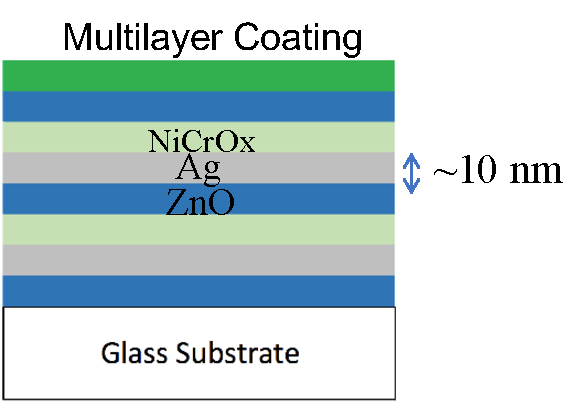
\includegraphics[width=0.75\linewidth]{Chap4/plots/Picture1a.pdf}}\label{Chap:Ag/ZnO:fig:1a}
\caption[Illustration of multi-layer structures and thin film morphology]{Illustration of multi-layer structures of architecture glass.}
  \label{Chap:Ag/ZnO:fig1}
\end{figure}
\endgroup

However, Ag/ZnO interface has weaker adhesion energy compared to many other metal/oxide interfaces. The strengths of adhesion between metals and oxides can largely affect the wetting behaviors and morphology of interfaces. On the other hand, defects, like islands forming, high surface roughness and high density of pinholes, will all reduce the satisfactory of glass quality, as shown in Liu's paper \cite{liu2013lithography}. For industrial practices, Ag thin film deposited on ZnO layers is usually above 10 nm thickness so as to guarantee continuous thin film. Therefore, to achieve continuous thin film with thinner layers can improve the cost efficiency by reducing the amount of Ag needed.

In this chapter, attention was paid to mainly two parts: 1) the effect of substrate on the Ag thin film quality; 2) the effect of alloy segregation at Ag grain boundary on the Ag thin film stability. \ac{GCMC} methods will be used to study the morphology of Ag thin film on different substrates with various substrate structures, lattice constant and bonding strength to Ag atoms. The goal of this study is to simulate the morphology after annealing, hence detailed kinetics, like bombardment effects, can be ignored. Therefore, \ac{GCMC} simulation will be a suitable tool, because it is based on the thermodynamic driving force. On the other hand, \ac{DFT} calculations will be used to study the segregation of alloy elements at different Ag grain boundaries.
\section{Customized Empirical Potential and GCMC Simulation Setup for Deposition}

\begingroup
\begin{figure}[!ht]
  \centering
  \subfigure{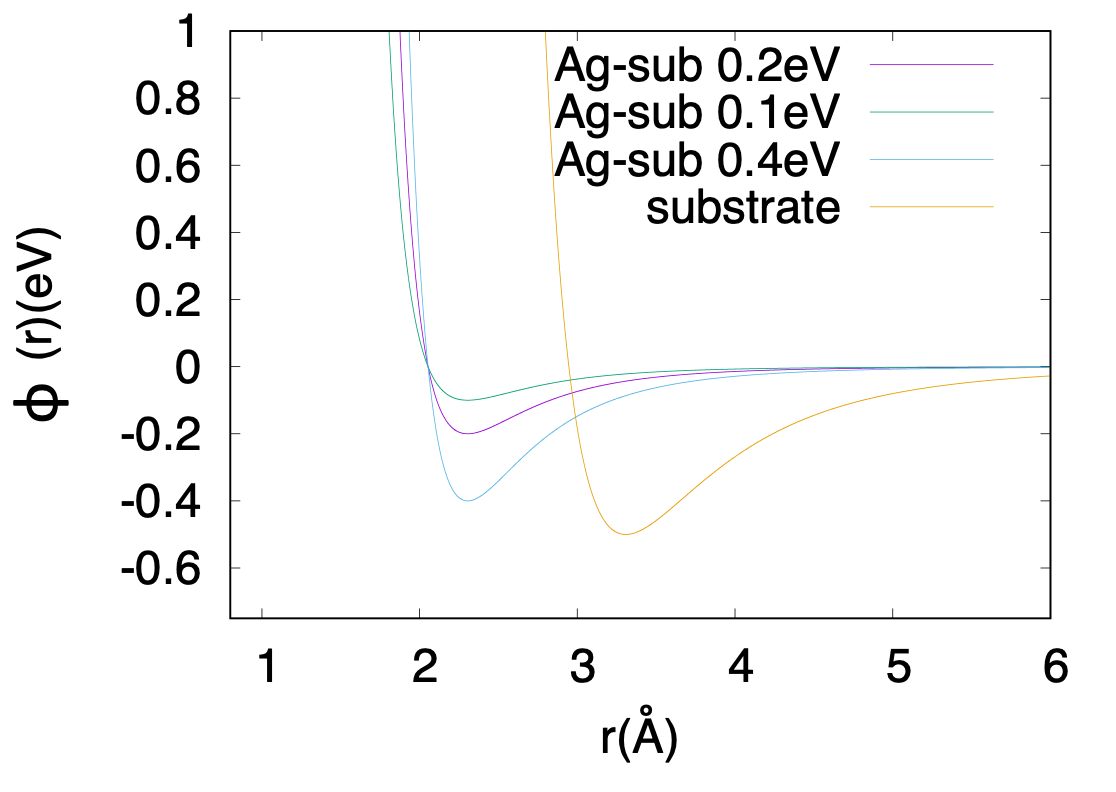
\includegraphics[width=0.9\linewidth]{Chap4/plots/Picture2.png}}
  \caption[Lennard-Jones potential used to describe different bonding strength and bond length of Ag-substrate atoms, and substrate-substrate atoms]{\ac{L-J} potential used to describe different bonding strength and bond length of Ag-substrate atoms, and substrate-substrate atoms.}
  \label{Chap:Ag/ZnO:fig2}
\end{figure}
\endgroup

In order to conduct \ac{GCMC} simulations accurately for metal deposition, a reasonable potential must be used to describe the interaction between Ag adsorbates and substrate atoms. An \ac{EAM} potential \cite{williams2016modeling} is used to describe the interaction between Ag-Ag atoms, while the interactions between Ag and substrate atoms need to be able to tuned for different bonding environments. As a result, we applied simple \ac{L-J} 12-6 potential \cite{jones1924determination} for Ag-substrate interaction and interactions between substrate-substrate atoms:
\begin{align}
 \Phi_{LJ} = 4\epsilon \left[ (\frac{\sigma}{r})^{12} - (\frac{\sigma}{r})^6\right]
 \label{Chap:Ag/ZnO:eq:LJ}
\end{align}
where, $\epsilon$ controls bonding strength and $\sigma$ changes equilibrium bond lengths. As shown in Fig. \ref{Chap:Ag/ZnO:fig2}, purple, green and blue lines describes the interaction between Ag atom and normal, week, and strong bonding with substrates, respectively. And the equilibrium bond length is fitted for the bond distance between Ag and ZnO substrates at $\sim$ 2.3$\angstrom$. And the yellow line corresponding to the substrate interactions itself, we set the bond length based on ZnO substrates lattice constant. And a strong potential well is used in order to simulate a more rigid substrate. The \ac{GCMC} code we used is from \cite{sina2017mapp}.

As we previously discussed in Chap. \ref{Chap:Mech:GCMC:GCMC}, the chemical potentials of elements of interest are used to decide the probability of accepting/rejecting a certain event. The Ag gas phase chemical potential is used, via:
\begin{align}
 \mu_{Ag(g)} = \mu_{Ag(bulk)} + k_{B}T\ln{\frac{p}{p_0}}
 \label{Chap:Ag/ZnO:eq:mu_Ag}
\end{align}
where, $p_0$ is the Ag evaporation pressure. Usually, the vacuum pressure of a sputtering chamber is $\sim$ 1 $pa$. So a chemical potential $\mu$ of -0.6 $eV$ is used to simulate $p$=1$Pa$ Ag partial pressure at 300$K$.

\begingroup
\begin{figure}[!ht]
  \centering
  \subfigure[]{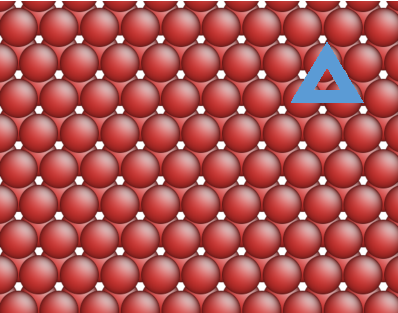
\includegraphics[width=0.49\linewidth]{Chap4/plots/Picture3a.pdf}}\label{Chap:Ag/W:fig:3a}
  \subfigure[]{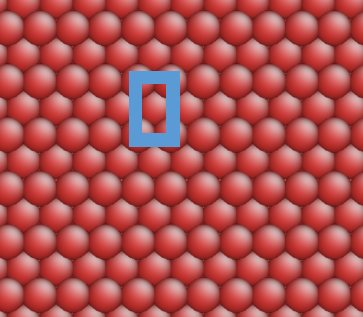
\includegraphics[width=0.44\linewidth]{Chap4/plots/Picture3b.pdf}}\label{Chap:Ag/W:fig:3b}
  \\
  \subfigure[]{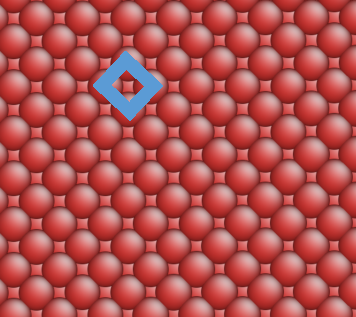
\includegraphics[width=0.44\linewidth]{Chap4/plots/Picture3c.pdf}}\label{Chap:Ag/W:fig:3c}
  \subfigure[]{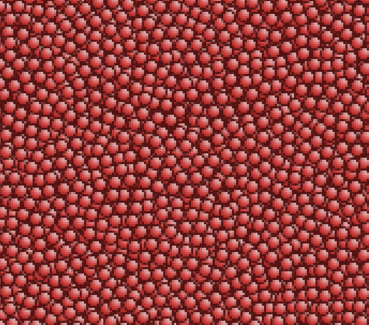
\includegraphics[width=0.44\linewidth]{Chap4/plots/Picture3d.pdf}}\label{Chap:Ag/W:fig:3d}
\caption[Four different substrate types for GCMC simulation.]{Four different substrate types for GCMC simulation: (a) hexagonal, (b) rectangular, (c) square like surface lattice, and (d) amorphous surface. }
  \label{Chap:Ag/W:fig3}
\end{figure}
\endgroup

Four different substrate types are used in this simulation, as shown in Fig. \ref{Chap:Ag/W:fig3}. Hexagonal surface unit, as shown in Fig. \ref{Chap:Ag/W:fig:3a}, corresponds to \ac{FCC} {111} surfaces and \ac{HCP} {0001} surfaces. Rectangular one, as shown in Fig. \ref{Chap:Ag/W:fig:3b}, corresponds to \ac{FCC} {110} surfaces and \ac{HCP} {10$\overline{1}$0} surfaces. Square one, as shown in Fig. \ref{Chap:Ag/W:fig:3c}, corresponds to \ac{FCC} {100} surfaces. Besides, an amorphous substrate, as shown in Fig. \ref{Chap:Ag/W:fig:3d}, is also created by quenching down from a high temperature. By combining different substrates with tunable \ac{L-J}, different substrates with different lattice constants can be achieved. Because \ac{FCC} and \ac{HCP} structures have different ways to calculate lattice constant, we will use bond length in the following sections to avoid confusion. By using strong and weak bonding of Ag-substrate interactions together, one can also simulate ``anchor'' sites on a regular substrates which will be discussed in subsection \ref{Chap:Ag/ZnO:section:anchor}.
\section{ZnO Substrate Yields the Best Ag Thin Film}

In this section, we will investigate which substrate type is best for Ag thin film deposition. Three different bond length will be used: 3.3$\angstrom$, 2.9$\angstrom$, 2.3$\angstrom$. 3.3$\angstrom$ is equivalent to ZnO lattice constant. 2.9$\angstrom$ is for Ag bond length, which means this substrate has a zero misfit for Ag thin film. At last, 2.3$\angstrom$ is selected for simulating a negative lattice mismatch factor, where lattice mismatch factor($f_{mismatch}$) is defined via:
\begin{align}
    f_{mismatch} = \frac{a_{substrate} - a_{film}}{a_{substrate}}
    \label{Chap:Ag/ZnO:eq:mismatch}
\end{align}

\section{Substrate ``Anchor'' Sites for Continuous Thin Film Morphology}
\label{Chap:Ag/ZnO:section:anchor}

As we mentioned before, random surface defects may have a positive effect on forming a continuous thin film. This may come from strong interactions between surface defect sites and Ag atoms. In this section, we will investigate the possibility of using the surface ``anchor'' site to improve the thin film continuity. A similar idea was initially proposed by Chambers et al. \cite{chambers2002laminar}. They considered the situation of transition metal getting oxidized and immobilized by the ZnO substrate. This is true when experiments are done in \ac{UHV}. But sputtering, especially industry-level sputtering usually happens in \ac{HV} conditions and the main source of oxygen is the residual gas which consists of water vapor as majorities as pointed out by Anders et al. \cite{anders2006smoothing} in 2006. In this section, a new criterion is proposed to search for stable anchor sites that can stand with water vapor and $\text{H}_{\text{2}}$ attacks. 

Therefore, we propose three criteria that are important for surface anchor elements: i) they can survive the attacks of water vapor($\text{H}_{\text{2}}\text{O}$) and $\text{H}_{\text{2}}$; ii) they have high diffusion barriers on saturated ZnO substrates; iii) they have strong bonding strength with Ag atoms.

For the first criterion, four different reactions are considered. The first two correspond to the two possible water ($\text{H}_{\text{2}}\text{O}$) dissociation reactions on the ZnO substrate with one ``anchor'' site, as shown in Fig. \ref{Chap:Ag/ZnO:fig:12a}. The upper reaction represents an incoming water molecule dissolve to one OH group attached to the ``anchor'' site and one H atom at a remote ``anchor'' site. The lower plot of Fig. \ref{Chap:Ag/ZnO:fig:12a}, represents the reaction of an incoming water molecule dissolve to one OH group attached to the ``anchor'' site and one H atom at a nearby O atom top. The third and fourth reaction corresponds to the two possible $\text{H}_{\text{2}}$ dissociation reactions on the ZnO substrate with one ``anchor'' site, as shown in Fig. \ref{Chap:Ag/ZnO:fig:12a}. We summarize the 4 reactions as below:
\begin{subequations}
\begin{align}
H_2O + 2 ZnO-X & \rightarrow ZnO-X-OH + ZnO-X-H
 \label{Chap:Ag/ZnO:eq:anchor1}\\
H_2O + ZnO-X & \rightarrow H-ZnO-X-OH
 \label{Chap:Ag/ZnO:eq:anchor2}\\
H_2 + 2 ZnO-X & \rightarrow ZnO-X-H + ZnO-X-H
 \label{Chap:Ag/ZnO:eq:anchor3}\\
H_2 + ZnO-X & \rightarrow H-ZnO-X-H
 \label{Chap:Ag/ZnO:eq:anchor4}
\end{align}
\end{subequations}


\newpage
\begingroup
\begin{figure}[!ht]
  \centering
  \subfigure[]{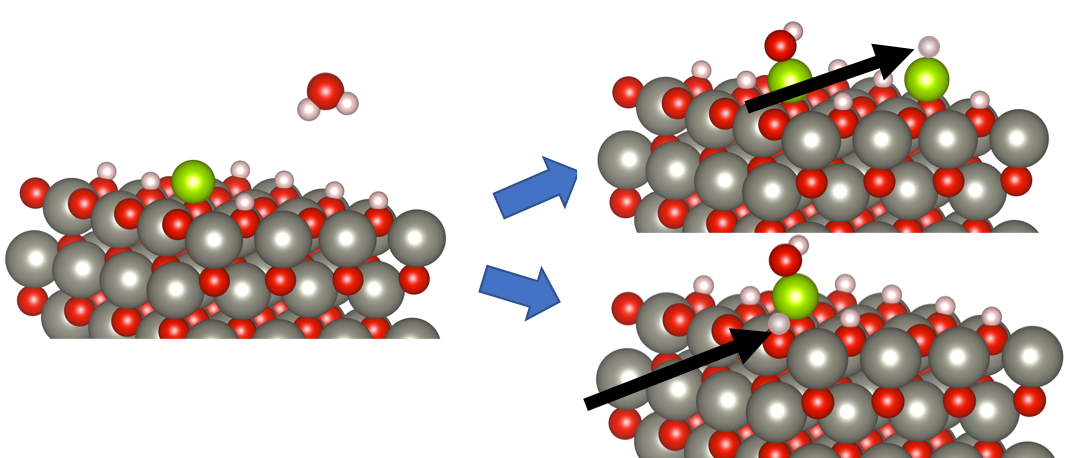
\includegraphics[width=0.85\linewidth]{Chap4/plots/Picture12a.png}}\label{Chap:Ag/ZnO:fig:12a}
  \subfigure[]{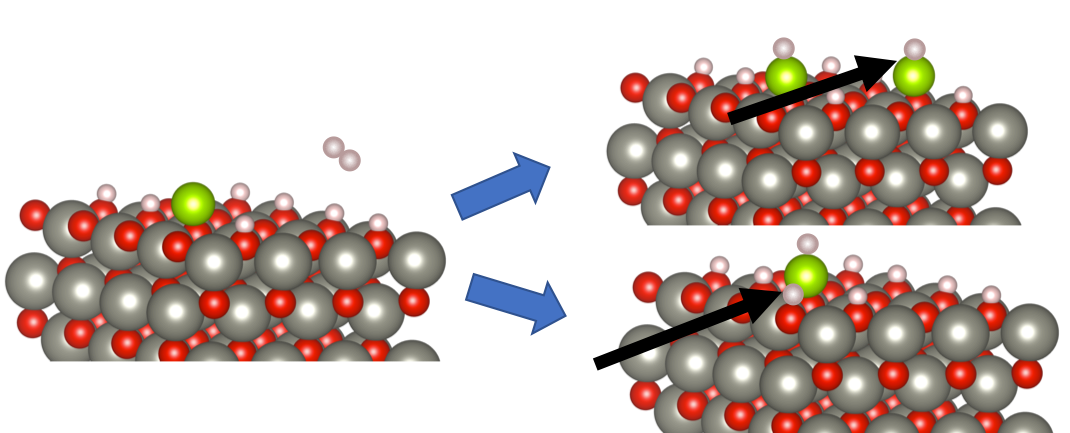
\includegraphics[width=0.85\linewidth]{Chap4/plots/Picture12b.png}}\label{Chap:Ag/ZnO:fig:12b}
\caption[Possible water and $\text{H}_{\text{2}}$ dissociation reactions on ZnO substrate with ``anchor'' sites.]{Possible water and $\text{H}_{\text{2}}$ dissociation reactions on ZnO substrate with one ``anchor'' site. (a) Two possible water ($\text{H}_{\text{2}}\text{O}$) dissociation reactions on ZnO substrate with anchor sites. (b) Two possible $\text{H}_{\text{2}}$ dissociation reactions on ZnO substrate with anchor sites. Red and grey atoms are O and Zn atoms, respectively. Green atoms represent the ``anchor'' element on ZnO substrate surfaces. Pink ones are H atoms.}
\label{Chap:Ag/ZnO:fig12}
\end{figure}
\endgroup

In order to have the ``anchor'' elements staying reactive on ZnO substrates, all the four equations need to yield positive enthalpies. After the screening the first criterion, as shown in Fig. \ref{Chap:Ag/ZnO:fig13}, Pd, Sb, Se, Sn, Cd, and Te can survive the environment of water and H. Cd is eliminated as it is an extremely toxic industrial and environmental pollutant. 

\begingroup
\begin{figure}[!ht]
  \centering
  \subfigure[]{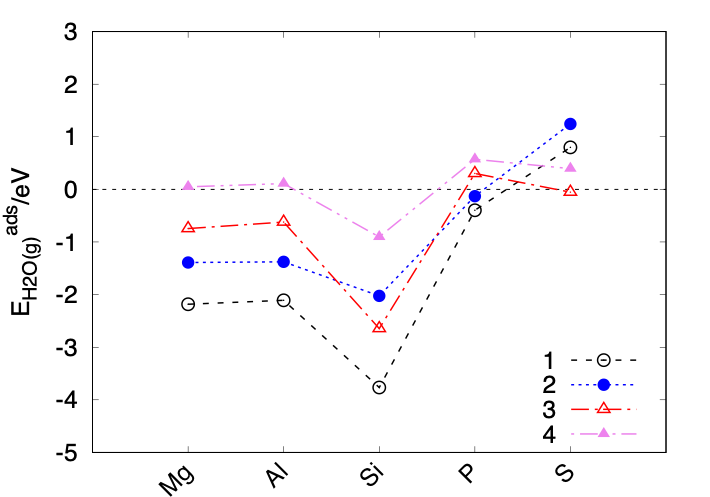
\includegraphics[width=0.45\linewidth]{Chap4/plots/Picture13a.png}}\label{Chap:Ag/ZnO:fig:13a}
  \subfigure[]{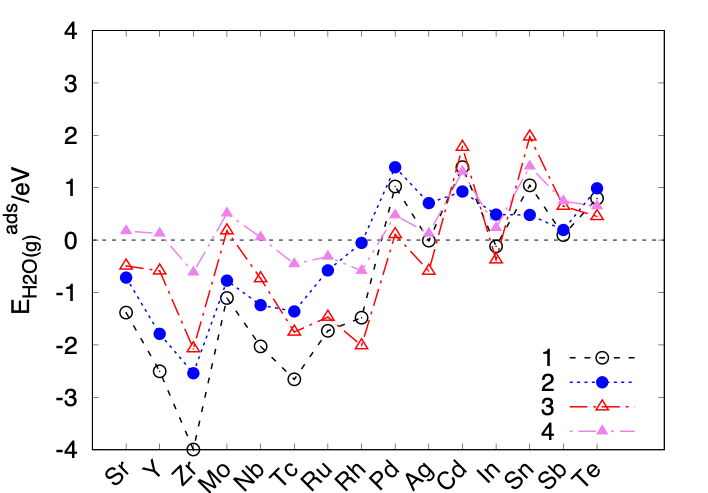
\includegraphics[width=0.45\linewidth]{Chap4/plots/Picture13b.png}}\label{Chap:Ag/ZnO:fig:13b}
  \\
  \subfigure[]{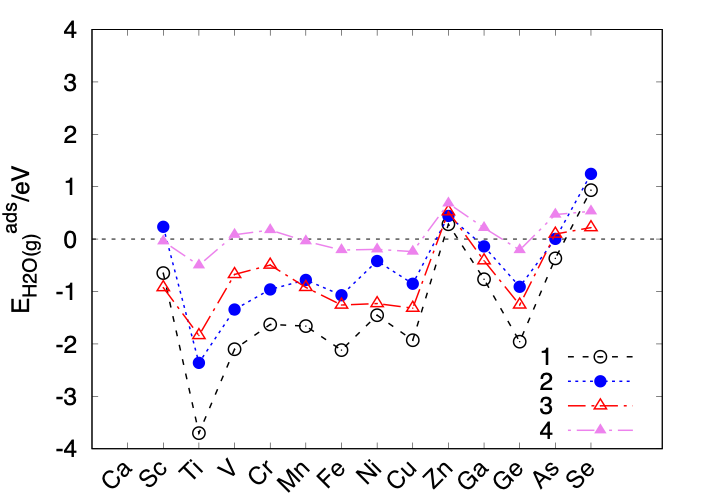
\includegraphics[width=0.45\linewidth]{Chap4/plots/Picture13c.png}}\label{Chap:Ag/ZnO:fig:13c}
  \subfigure[]{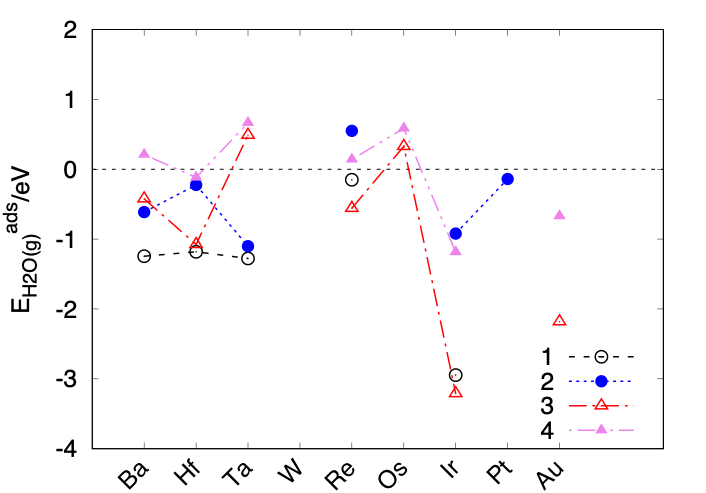
\includegraphics[width=0.45\linewidth]{Chap4/plots/Picture13d.png}}\label{Chap:Ag/ZnO:fig:13d}
\caption[Water and $\text{H}_{\text{2}}$ dissociation reactions energies on ZnO substrate with ``anchor'' sites.]{Water and $\text{H}_{\text{2}}$ dissociation reactions energies on ZnO substrate with ``anchor'' sites. Reaction 1 and 2 corresponds to 2 possible water dissociation reactions in Fig.
\ref{Chap:Ag/ZnO:fig:12a}, respectively. Reaction 3 and 4 corresponds to 2 possible $\text{H}_{\text{2}}$ dissociation reactions in Fig. \ref{Chap:Ag/ZnO:fig:12b}, respectively.}
\label{Chap:Ag/ZnO:fig13}
\end{figure}
\endgroup

\begin{table}[!ht]
\caption[``Anchor'' elements diffusion barriers on ZnO saturated with $\frac{1}{2}$ \ac{ML} H.]{``Anchor'' elements diffusion barriers on ZnO saturated with $\frac{1}{2}$ \ac{ML} H.}
\label{Chap:Ag/ZnO:tab1}
\centering
\begin{tabular}{cc}
\\
\hline
\hline
Substrate & \begin{tabular}[c]{@{}c@{}}Diffusion barrier on ZnO saturated\\ with $\frac{1}{2}$ \ac{ML} H [eV]\end{tabular} \\ \hline
Ag        & 0.077                                                                                                          \\
Pd        & 0.275                                                                                                          \\
Sb        & 0.111                                                                                                          \\
Se        & 1.338                                                                                                          \\
Sn        & 0.341                                                                                                          \\
Te        & 0.999                                                                                                          \\ \hline
\hline
\end{tabular}
\end{table}

For the second and third criteria, all the 5 elements have orders higher diffusion barriers compared to Ag atoms on fully-saturated ZnO substrates, as shown in Table. \ref{Chap:Ag/ZnO:tab1}. Moreover, as we can see from Table. \ref{Chap:Ag/ZnO:tab2}, all the 5 elements have much stronger bonding strengths to an Ag atom compared to bare ZnO substrates as well.

\begin{table}[!ht]
\caption[Ag adsorption on saturated ZnO substrate with ``anchor'' sites.]{Ag adsorption on saturated ZnO substrate with ``anchor'' sites.}
\label{Chap:Ag/ZnO:tab2}
\centering
\begin{tabular}{cc}
\\
\hline
\hline
Substrate              & Adsorption energy(eV) \\ \hline
ZnO with $\frac{1}{2}$ \ac{ML}    & -0.716                \\
Pd & -1.716                \\
Sb & -2.242                \\
Se & -2.055                \\
Sn & -2.284                \\
Te & -1.931                \\ \hline
\hline
\end{tabular}
\end{table}

In order to demonstrate the effect of surface ``anchor'' sites on Ag thin film morphology, \ac{GCMC} simulations are conducted. 0.05 \ac{ML} of substrate atoms are randomly changed to ``anchor'' site atoms which has a stronger binding to Ag. Then 10 \ac{ML} of Ag atoms are deposited. In Figure. \ref{Chap:Ag/ZnO:fig14}, a much continuous Ag thin film can be seen with 0.05 \ac{ML} of ``anchor'' sites. With randomly distributed ``anchor'' sites, more nuclei can be achieved, hence more continuous ultra-thin film.

\newpage
\begingroup
\begin{figure}[!ht]
  \centering
  \subfigure[]{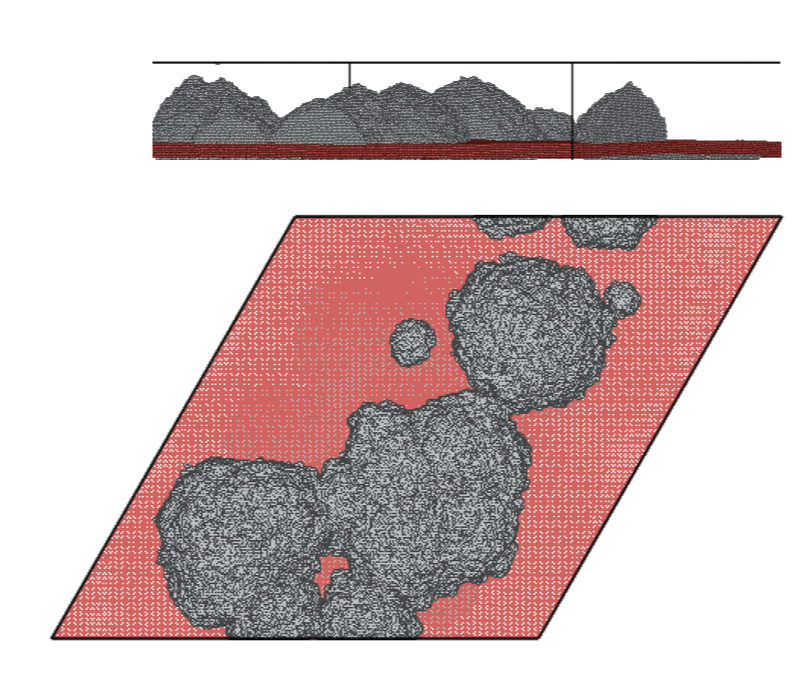
\includegraphics[width=0.65\linewidth]{Chap4/plots/Picture14a.png}}\label{Chap:Ag/ZnO:fig:14a}
  \subfigure[]{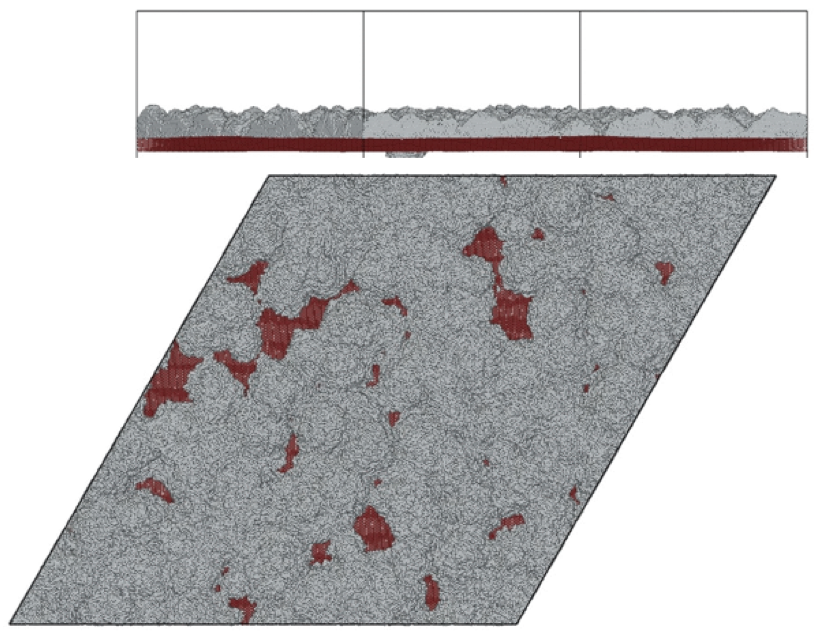
\includegraphics[width=0.65\linewidth]{Chap4/plots/Picture14b.png}}\label{Chap:Ag/ZnO:fig:14b}
\caption[GCMC simulation results for 10 \ac{ML} Ag deposition on ZnO with and without 0.05\ac{ML} surface ``anchor'' sites.]{\ac{GCMC} simulation results for 10 \ac{ML} Ag deposition on ZnO with and without 0.05\ac{ML} surface ``anchor'' sites. (a) Ag island growth pattern on ZnO without surface ``anchor'' sites. (b) Ag island growth pattern on ZnO with 0.05\ac{ML} surface ``anchor'' sites.}
\label{Chap:Ag/ZnO:fig14}
\end{figure}
\endgroup
\section{Alloy Segregation at Grain Boundary to Stabilize Polycrystalline  Thin Film}
\label{Chap:Ag/ZnO:GB}


%The interactions between solute atoms and crystalline defects such as dislocations, and grain boundaries play an essential role in determining the physical, chemical and mechanical properties of solid-solution alloys. In recent years, the ability to predict solute segregation at high symmetry grain boundaries from first principles have been widely studied. However, previous algorithms have mainly focused on the simple grain boundary structures for dilute solute cases due to the costly computation power needed by density functional theory (DFT). Here, we present a general atomistic approach to optimize the structures and simulate solute segregation trends of grain boundaries in multiple component systems by the combination of a highly efficient genetic algorithm and the grand canonical ensemble, in which components are not restricted to dilute or stoichiometric cases. Different chemical potential can be used as input for creating different reservoirs for the grain boundary phases. In our study, thousands-atom grain boundary systems will be investigated by well-established empirical potentials (MEAM or EAM potentials) for Mg-based alloy systems, like Mg-Y or Mg-Zn, which are potential candidates for lightweight structural components as a result of their low density and high specific strength. Because of the complicated potential energy landscapes (PEL) coming from both geometric and occupational freedom, we will either average a good amount of small configurations by Boltzmann statistics based on their energy distributions for patterned segregation systems or use a large supercell to study cluster segregation systems across the grain boundaries. Final structures will then be used to investigate the effect of solute on mechanical behaviors of grain boundary systems.

During the heat treatment of multi-layer coating structures, quality problems like discontinuous thin films, change of colors can happen. The grain boundary grooving effect, as shown in Fig. \ref{Chap:Ag/ZnO:fig15}, results in those voids and discontinuous films that degrade the quality of thin films. \cite{mullins1957theory,simrick2012thermal} This grain boundary grooving effect will increase with larger grain sizes. \cite{martin2009thermal} Therefore, we can try to stabilize grain sizes of nanocrystalline alloys by doping during heat treatment. \cite{chookajorn2012design,jiao2018nanocrystalline}


\begingroup
\begin{figure}[!ht]
  \centering
  \subfigure{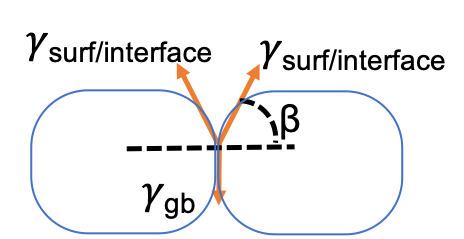
\includegraphics[width=0.65\linewidth]{Chap4/plots/Picture15.png}}
  \caption[Illustration of grain boundary grooving effects.]{Illustration of grain boundary grooving between two grains. The blue solid circle-like shape indicate grains. $\beta$ is the dihedral angle. $\gamma_{surf/interface}$, $\gamma_{gb}$ are the surface/interface energy and grain boundary energy, respectively.}
  \label{Chap:Ag/ZnO:fig15}
\end{figure}
\endgroup


Solute atoms, whether they are added voluntarily for specific needs, inevitably remained as impurities after the synthesis, or introduced during the service of the material, can affect various properties of alloys by changing the stability and mobility of crystalline defects, like grain boundaries. In this section, we tried to add trace amounts of alloying elements to stabilize grain boundaries. From experiments and phenological model, W should segregate at Ag grain boundaries. \cite{chookajorn2012design,jiao2018nanocrystalline} We used \ac{DFT} to search for potential candidates. Simple grain boundaries like $\Sigma$5 (310), $\Sigma$3 (112) and $\Sigma$3 (111) are used. We defined the segregation energy $E_{seg}$ via,
\begin{align}
E_{seg} = E_{X near GB} - E_{X away from GB}
 \label{Chap:Ag/ZnO:eq:gb_seg}
\end{align}
where $E_{X near GB}$ and $E_{X away from GB}$ are energy when solute atoms are located close to and away from the grain boundary, respectively, for example, as shown in Fig. \ref{Chap:Ag/ZnO:fig16}.


\begingroup
\begin{figure}[!ht]
  \centering
  \subfigure{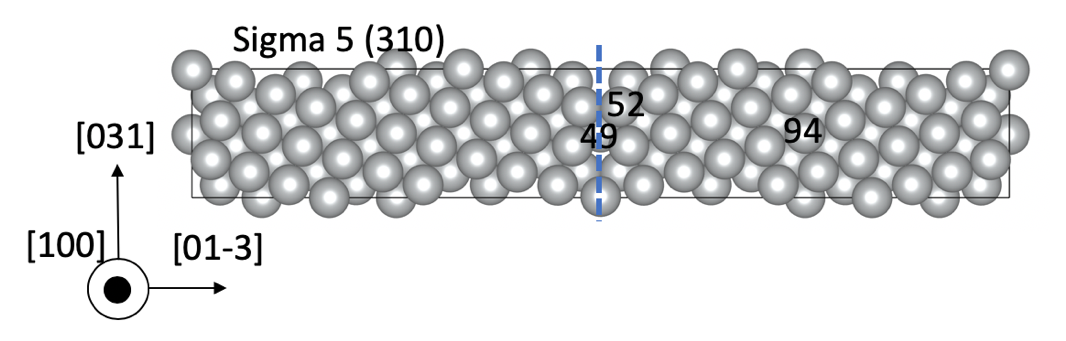
\includegraphics[width=1.0\linewidth]{Chap4/plots/Picture16.png}}
  \caption[Atomistic structure of $\Sigma$5 (310) Ag grain boundary.]{Atomistic structure of $\Sigma$5 (310) Ag grain boundary. The blue vertical line indicates where the grain boundary is. Because of a periodic boundary condition is used, there is another grain boundary at the end of the simulation box. Atom labeled with \#49, 51 and 94 are two atoms close to the grain boundary and far away from grain boundary, respectively.}
  \label{Chap:Ag/ZnO:fig16}
\end{figure}
\endgroup


All-electron \ac{PAW} potentials were employed for the elemental constituents with the \ac{GGA} of \ac{PBE} for the exchange-correlation energy functional, $\mu_{xc}$, and the interpolation formula of Vosko et al. \cite{vosko1980accurate}. Using plane-wave cutoff energy of at 450.0 eV, the total energy for all models of initial and final images was converged to $10^{−7}$ eV/cell. The reciprocal space of bulk supercells was sampled with (2x1x5), (10x1x4), and (5x3x1) k-point grids for atomic structures of $\Sigma$5 (310), $\Sigma$3 (112) and $\Sigma$3 (111). Each grid was generated using the Gamma scheme.


\begingroup
\begin{figure}[!ht]
  \centering
  \subfigure[]{
\includegraphics[width=0.49\linewidth]{Chap4/plots/Picture17a.png}}
  \subfigure[]{
\includegraphics[width=0.49\linewidth]{Chap4/plots/Picture17b.png}}
  \subfigure[]{
\includegraphics[width=0.49\linewidth]{Chap4/plots/Picture17c.png}}
\caption[Segregation energies of different elements at $\Sigma$5 (310) grain boundary.]{Segregation energies of different elements at $\Sigma$5 (310) grain boundary. The solid circles are for elements segregated at location \#49 in Fig. \ref{Chap:Ag/ZnO:fig16}. And the open triangles are for elements segregated at location \#52 in Fig. \ref{Chap:Ag/ZnO:fig16}. Sub-figure (a), (b), and (c) show d-elements and some p-elements in fourth, fifth, and sixth periods, respectively.}
\label{Chap:Ag/ZnO:fig17}
\end{figure}
\endgroup


A double grain boundary periodic supercell was used for constructing a $\Sigma$5 (310) grain boundary, as shown in Fig. \ref{Chap:Ag/ZnO:fig16}. Atom \#49, 52 were chosen to be atoms close to the grain boundary. And atom \#94 was chosen to be the atom far away from grain boundary. We calculated the grain boundary segregation energies for different elements in Fig. \ref{Chap:Ag/ZnO:fig17}. Their segregation across the period shows a consistent trend, which is that the segregation energy increases at first and then drops. A naive explanation would be the competition between the d-electron orbital filling and the effects of the volume as atomic size increases. However, these results are contradictory to the experimental values in terms of the element tungsten, W. \cite{chookajorn2012design,jiao2018nanocrystalline} In Figure. \ref{Chap:Ag/ZnO:fig18} and \ref{Chap:Ag/ZnO:fig19}, other grain boundaries like $\Sigma$3 (112) and $\Sigma$3 (111), are also investigated using \ac{DFT}, and no case show W will segregate at either of those types of grain boundaries, despite a similar trend holds true for all of the three simple grain boundaries.

\begingroup
\begin{figure}[!ht]
  \centering
  \subfigure[]{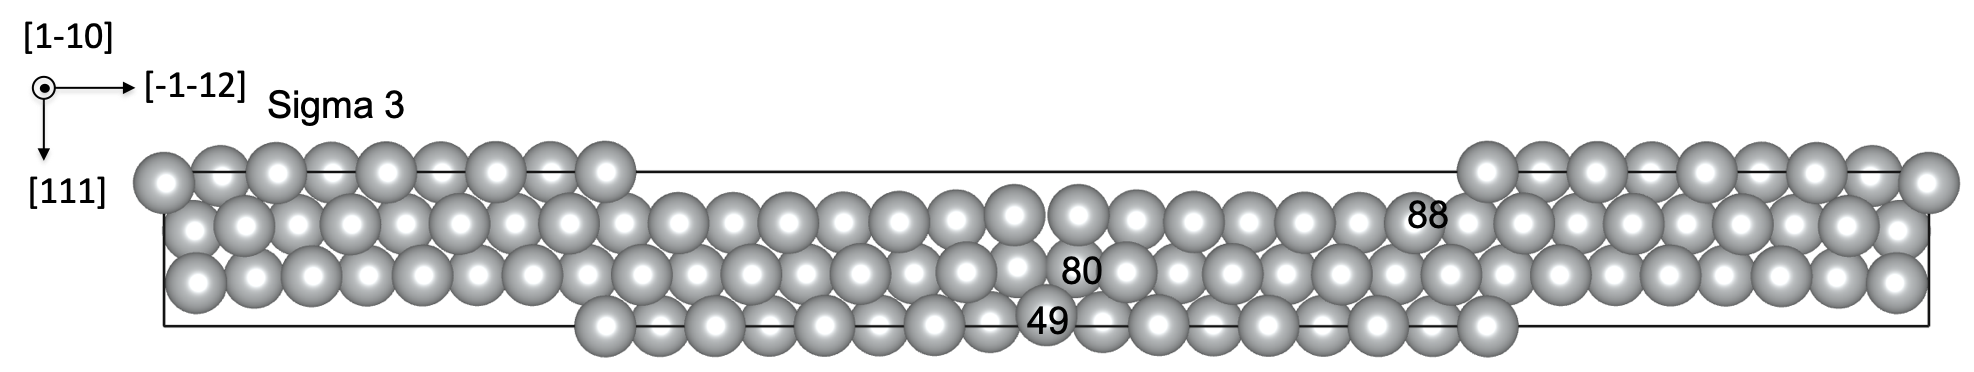
\includegraphics[width=1.0\linewidth]{Chap4/plots/Picture18.png}}
  \subfigure[]{
\includegraphics[width=0.49\linewidth]{Chap4/plots/Picture18a.png}}
  \subfigure[]{
\includegraphics[width=0.49\linewidth]{Chap4/plots/Picture18b.png}}
  \subfigure[]{
\includegraphics[width=0.49\linewidth]{Chap4/plots/Picture18c.png}}
\caption[Segregation energies of different elements at $\Sigma$3 (112) grain boundary.]{Segregation energies of different elements at $\Sigma$3 (112) grain boundary. The solid circles are for elements segregated at location \#49 in (a). And the open triangles are for elements segregated at location \#80. Sub-figure (b), (c), and (d) show d-elements and some p-elements in fourth, fifth, and sixth periods, respectively.}
\label{Chap:Ag/ZnO:fig18}
\end{figure}
\endgroup

\begingroup
\begin{figure}[!ht]
  \centering
  \subfigure[]{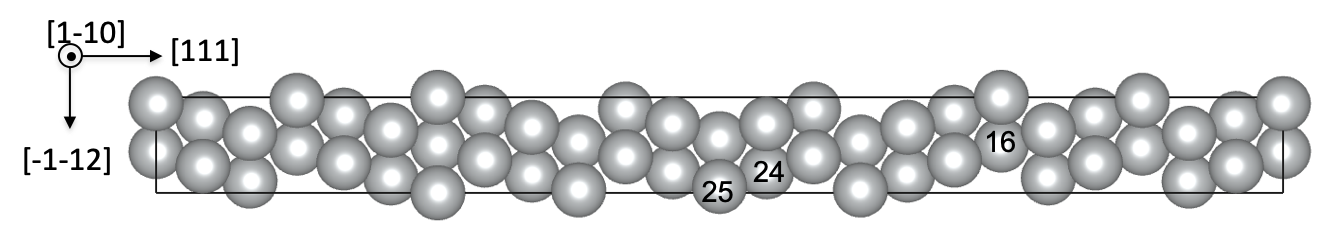
\includegraphics[width=1.0\linewidth]{Chap4/plots/Picture19.png}}
  \subfigure[]{
\includegraphics[width=0.49\linewidth]{Chap4/plots/Picture19a.png}}
  \subfigure[]{
\includegraphics[width=0.49\linewidth]{Chap4/plots/Picture19b.png}}
  \subfigure[]{
\includegraphics[width=0.49\linewidth]{Chap4/plots/Picture19c.png}}
\caption[Segregation energies of different elements at $\Sigma$3 (111) grain boundary.]{Segregation energies of different elements at $\Sigma$3 (111) grain boundary. The solid circles are for elements segregated at location \#24 in (a). And the open triangles are for elements segregated at location \#25. Sub-figure (b), (c), and (d) show d-elements and some p-elements in fourth, fifth, and sixth periods, respectively.}
\label{Chap:Ag/ZnO:fig19}
\end{figure}
\endgroup


A more complicated grain boundary, $\Sigma$29 (520), from literature \cite{zhu2018predicting} as shown in Fig. \ref{Chap:Ag/ZnO:fig20}, was also studied, and it still shows repulsive interactions for W. In Table. \ref{Chap:Ag/ZnO:tab3}, W segregation energy at different sites was listed. All of them show positive values except site \# 196. However, when W atom was placed at that site, large distortion was observed across the grain boundary. And it was not a fair comparison to see W will segregate at that specific site \#196.  Traditionally, researchers first obtained relaxed grain boundary structures from pure metals and then substitute dilute atoms to calculate alloy segregation effects. One possibility of the discrepancy we observed could be that alloying elements can not only change the chemistry of the grain boundaries but also change the atomistic structure of grain boundaries in alloys. Besides, in reality, more complicated grain boundaries, like grain boundary complexions, exist. \cite{cantwell2014grain} Therefore, more complicated grain boundary structures need to be obtained by global optimization methods, e.g. evolutionary algorithm, to investigate the alloy segregation effects.


\begingroup
\begin{figure}[!ht]
  \centering
  \subfigure{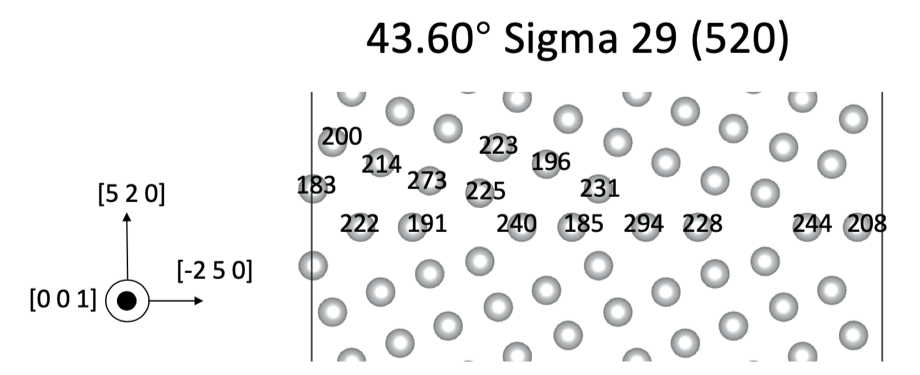
\includegraphics[width=0.8\linewidth]{Chap4/plots/Picture20.png}}
  \caption[Atomistic structure of $\Sigma$29 (520) Ag grain boundary.]{Atomistic structure of $\Sigma$29 (520) Ag grain boundary. The blue vertical line indicates where the grain boundary is.}
  \label{Chap:Ag/ZnO:fig20}
\end{figure}
\endgroup

\begin{table}[!ht]
\caption[Tungsten segregation energy $E_{seg}$ at different sites of Ag $\Sigma$29 (520) grain boundary.]{Tungsten segregation energy $E_{seg}$ at different sites of $\Sigma$29 (520) Ag grain boundary. The segregation energy $E_{seg}$ was calculated via Equation. \ref{Chap:Ag/ZnO:eq:gb_seg}.}
\label{Chap:Ag/ZnO:tab3}
\centering
\begin{tabular}{cc}
\hline
\hline
site & $E_{seg}$ eV/Atom \\ 
\hline
183  & .17150937         \\
185  & .39017180         \\
191  & .33935043         \\
196  & -.01991584        \\
200  & .10469391         \\
208  & .45059809         \\
214  & .02440580         \\
222  & .42554973         \\
223  & .12724989         \\
225  & .26205663         \\
228  & .38927174         \\
231  & .11203458         \\
240  & .51875226         \\
244  & .55923929         \\
273  & .18312458         \\
294  & .42944364         \\ 
\hline
\hline
\end{tabular}
\end{table}
\section{Conclusions}
In this chapter, we studied how does substrate affect Ag thin film morphology by using \ac{GCMC} and empirical potentials. This method is expandable to other metal thin films as well as other substrates, like MgO.

We found that only Ag films on the hexagonal substrate are robust to substrate lattice constant and bonding strength changes, and yields most \{111\} orientation Ag. Therefore, Ag thin film quality (improve texture and reduce internal defects) can be improved by increasing ZnO substrate quality. 

In order to achieve more continuous Ag thin films with less Ag, some elements can be added as ``anchor'' sites to incoming Ag atoms. Pd, Sb, Se, Sn, and Te can be good candidates as ``anchor'' sites on the ZnO substrate. With trace amount (0.05\ac{ML}) of ``anchor'' sites on the substrate, more nuclei can be achieved, hence more continuous ultra-thin film.

We also tried to search doping elements that can segregate in Ag grain boundaries to stabilize grain size during heat treatments. First-principles calculation showed transition metals, e.g. W, do not segregation in Ag grain boundaries, which is inconsistent with experiments. We suspect that alloying elements can not only change chemistry of the grain boundaries, but also disrupt the atomistic structure of grain boundaries in alloys. Therefore, an evolutionary algorithm to search stable complex grain boundaries for binary alloy need to be used. Besides, the electronic mechanism also needs to be investigated.